\subsection{Petri net editor}
\writer{Albert}

The Petri net editor is a component which consists of an extension of the ePNK editor. It contains all the functionality that ePNK provides and also adds the features described previously in this document, and that can be summarized in Figure \ref{fig:uml-petrinet-editor}. Its actual implementation is shown in Figure \ref{fig:petri-net-domain-model}.

\begin{figure}[htp]
\begin{center}
  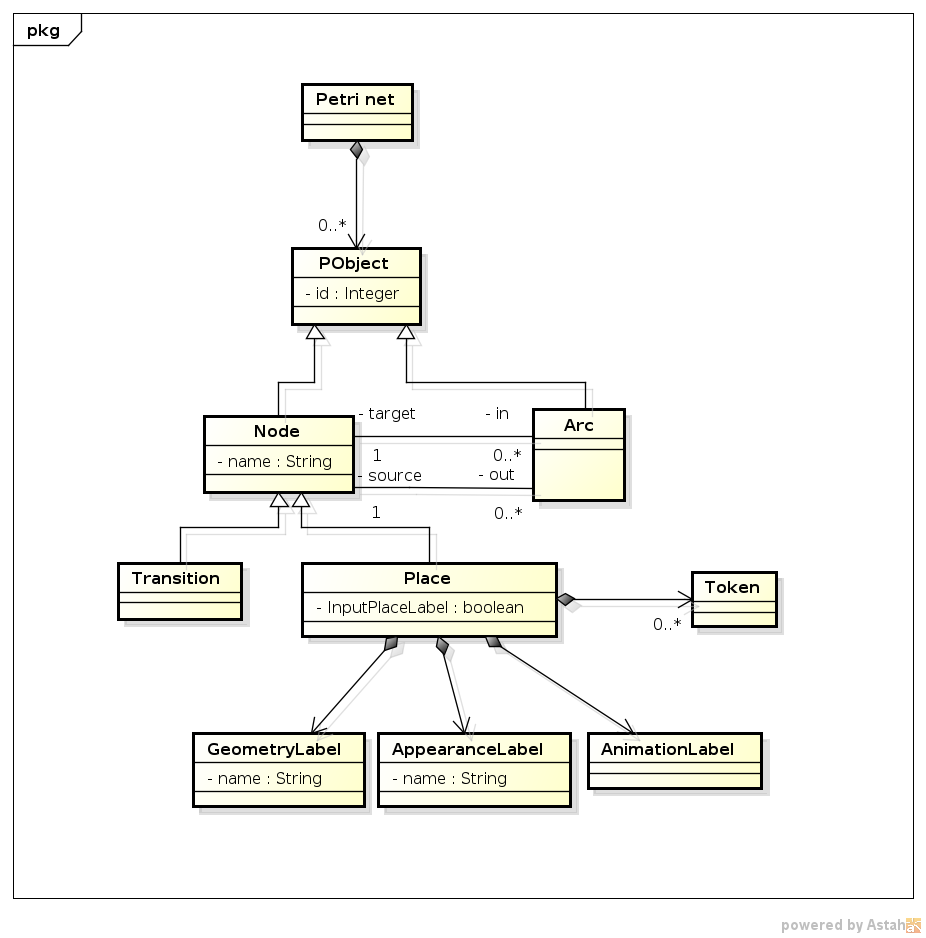
\includegraphics[width=0.6\textwidth]{image/petrinet_uml.png}
  \caption{UML for the Petri net Editor}
  \label{fig:uml-petrinet-editor}
\end{center}
\end{figure}

\begin{figure}[htp]
\begin{center}
  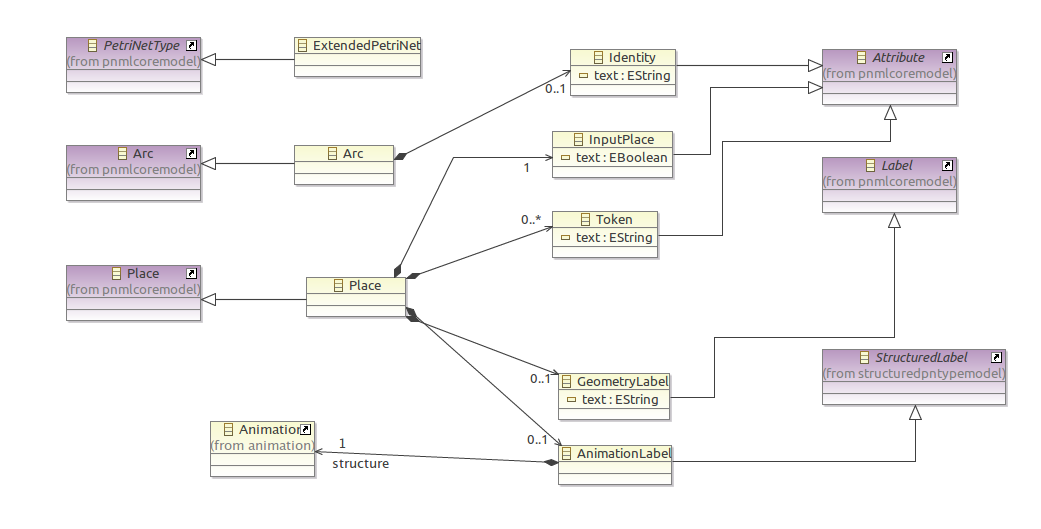
\includegraphics[width=0.8\textwidth]{image/petrinet_editor_domain.png}
  \caption{Petri net editor domain model}
  \label{fig:petri-net-domain-model}
\end{center}
\end{figure}

\subsubsection{Petri net editor classes}

A description of the classes shown in Figure \ref{fig:petri-net-domain-model} is provided.

\paragraph{Place}

The class Place extends from Place in the \textit{pnmlcoremodel}, and contains the following attributes:

\begin{itemize}
	\item \textbf{Token}: an ePNK string label to indicate the presence of one or more tokens in this Place.
	\item \textbf{AppearanceLabel}: an ePNK string label to indicate the shape and texture of the Place.
	\item \textbf{InputPlaceLabel}: an ePNK boolean attribute to indicate if the place is interactive for the user or not (if tokens can be added in runtime by the user).
	\item \textbf{GeometryLabel}: an ePNK string label to indicate the geometry location of the Place in the simulation.
	\item \textbf{AnimationLabel}: : an ePNK structured label which contains an Animation object and that contains all the information of the animation or sequence of animations executed when a Token is in this Place.
\end{itemize}

\paragraph{Arc}

The class Arc extends from Arc in the \textit{pnmlcoremodel}, and contains the following attributes:

\begin{itemize}
	\item \textbf{Identity}: an ePNK integer label to indicate the id of an arc, which is required for proper visualization of the Token "movement" during the simulation.
\end{itemize}